%!TEX program = xelatex
\documentclass{beamer}

\usepackage{booktabs}
\usepackage{pifont}
\usepackage{rotating}
\usepackage{appendixnumberbeamer}
\usepackage[caption=false]{subfig}
\usepackage{siunitx}
\usepackage{pgfplots}
\pgfplotsset{compat=newest}
\usepackage{pgfplotstable}
\usetikzlibrary{plotmarks,arrows}
\tikzset{>=latex}

\usetheme{Execushares}

\title{Numerical Characterization of Ultrasound Elastography for the Early Detection of Deep Tissue Injuries}
\subtitle{A thesis submitted in partial fulfilment of the requirements for the degree of Master of Science}
\author{Kenton David Hamaluik}
\institute{University of Alberta}
\date{June 23, 2014}

\newcommand{\rotHead}[1]{\begin{rotate}{60}#1\end{rotate}}
\newcommand{\cmark}{\color{ExecusharesBlue}\ding{51}}
\newcommand{\xmark}{\color{ExecusharesRed}\ding{55}}
\newcommand{\percent}{\%}

\definecolor{pc1}{HTML}{8DD3C7}
\definecolor{pc2}{HTML}{FDB462}
\definecolor{pc3}{HTML}{FB8072}
\definecolor{pc4}{HTML}{80B1D3}
\definecolor{pc5}{HTML}{B3DE69}
\definecolor{pc6}{HTML}{BEBADA}
\definecolor{pc7}{HTML}{FCCDE5}
\definecolor{pc8}{HTML}{D9D9D9}
\definecolor{pc9}{HTML}{FFFFB3}
\pgfplotscreateplotcyclelist{ColourPlotCycle}{%
only marks,mark options=solid,solid,ultra thick,pc1,every mark/.append style={fill=pc1},mark=o\\%
only marks,mark options=solid,dashed,ultra thick,pc2,every mark/.append style={fill=pc2},mark=square\\%
only marks,mark options=solid,dotted,ultra thick,pc3,every mark/.append style={fill=pc3},mark=diamond*\\%
only marks,mark options=solid,dashdotted,ultra thick,pc4,every mark/.append style={fill=pc4},mark=pentagon*\\%
only marks,mark options=solid,dash pattern=on 4pt off 1pt on 4pt off 4pt,ultra thick,pc5,every mark/.append style={fill=pc5},mark=triangle*\\%
only marks,mark options=solid,solid,ultra thick,pc6,every mark/.append style={fill=pc6},mark=*\\%
only marks,mark options=solid,dashed,ultra thick,pc7,every mark/.append style={fill=pc7},mark=square*\\%
only marks,mark options=solid,dotted,ultra thick,pc8,every mark/.append style={fill=pc8},mark=diamond\\%
only marks,mark options=solid,dashdotted,ultra thick,pc9,every mark/.append style={fill=pc9},mark=pentagon\\%
}
\pgfplotscreateplotcyclelist{ColourPlotRegressionCycle}{%
only marks,solid,ultra thick,pc1,every mark/.append style={fill=pc1},mark options=solid,mark=o\\%
solid,ultra thick,pc1\\%
only marks,dashed,ultra thick,pc2,every mark/.append style={fill=pc2},mark options=solid,mark=square\\%
dashed,ultra thick,pc2\\%
only marks,dotted,ultra thick,pc3,every mark/.append style={fill=pc3},mark options=solid,mark=diamond*\\%
dotted,ultra thick,pc3\\%
only marks,dashdotted,ultra thick,pc4,every mark/.append style={fill=pc4},mark options=solid,mark=pentagon*\\%
dashdotted,ultra thick,pc4\\%
only marks,dash pattern=on 4pt off 1pt on 4pt off 4pt,ultra thick,pc5,every mark/.append style={fill=pc5},mark options=solid,mark=triangle*\\%
dash pattern=on 4pt off 1pt on 4pt off 4pt,ultra thick,pc5\\%
only marks,solid,ultra thick,pc6,every mark/.append style={fill=pc6},mark options=solid,mark=*\\%
solid,ultra thick,pc6\\%
only marks,dashed,ultra thick,pc7,every mark/.append style={fill=pc7},mark options=solid,mark=square*\\%
dashed,ultra thick,pc7\\%
only marks,dotted,ultra thick,pc8,every mark/.append style={fill=pc8},mark options=solid,mark=diamond\\%
dotted,ultra thick,pc8\\%
only marks,dashed,ultra thick,pc9,every mark/.append style={fill=pc9},mark options=solid,mark=pentagon\\%
solid,ultra thick,pc9\\%
}
\pgfplotscreateplotcyclelist{SmoothColourPlotCycle}{%
solid,ultra thick,pc1\\%
dashed,ultra thick,pc2\\%
dotted,ultra thick,pc3\\%
dashdotted,ultra thick,pc4\\%
dash pattern=on 4pt off 1pt on 4pt off 4pt,ultra thick,pc5\\%
solid,ultra thick,pc6\\%
dashed,ultra thick,pc7\\%
dotted,ultra thick,pc8\\%
dashdotted,ultra thick,pc9\\%
}
\pgfplotscreateplotcyclelist{BarColourPlotCycle}{%
fill=pc1\\%
fill=pc2\\%
fill=pc3\\%
fill=pc4\\%
fill=pc5\\%
fill=pc6\\%
fill=pc7\\%
fill=pc8\\%
fill=pc9\\%
}

\definecolor{RdBuWhiteGrey}{RGB}{247,247,247}
\pgfplotsset{
	colormap={RdBu}{
		rgb255(0cm)=(5,48,97);
		rgb255(1cm)=(33,102,172);
		rgb255(2cm)=(67,147,195);
		rgb255(3cm)=(146,197,222);
		rgb255(4cm)=(209,229,240);
		rgb255(5cm)=(247,247,247);
		rgb255(6cm)=(253,219,199);
		rgb255(7cm)=(244,165,130);
		rgb255(8cm)=(214,96,77);
		rgb255(9cm)=(178,24,43);
		rgb255(10cm)=(103,0,31);
	}
}
\pgfplotsset{
	colormap={YlOrRd}{
		rgb255(0cm)=(128,0,38);
		rgb255(1cm)=(189,0,38);
		rgb255(2cm)=(227,26,28);
		rgb255(3cm)=(252,78,42);
		rgb255(4cm)=(253,141,60);
		rgb255(5cm)=(254,178,76);
		rgb255(6cm)=(254,217,118);
		rgb255(7cm)=(255,237,160);
		rgb255(8cm)=(255,255,204);
	}
}

\pgfmathdeclarefunction{gauss}{3}{%
  \pgfmathparse{1/(#2*sqrt(2*pi))*exp(-((#3-#1)^2)/(2*#2^2))}%
}

\begin{document}
	\setcounter{showProgressBar}{0}
	\setcounter{showSlideNumbers}{0}

	\frame{\titlepage}

	\begin{frame}
		\frametitle{Contents}
		\begin{enumerate}
			\item Introduction \\ \textcolor{ExecusharesGrey}{\footnotesize\hspace{1em} The reasons for and goals of this research}
			\item Quasi-Static Ultrasound Elastography (\alert{QS USE}) \\ \textcolor{ExecusharesGrey}{\footnotesize\hspace{1em} Estimating stiffness using manual palpation}
			\item Acoustic Radiation Force Impulse (\alert{ARFI}) Imaging \\ \textcolor{ExecusharesGrey}{\footnotesize\hspace{1em} Using transducer-generated forces instead of manual palpation}
			\item Shear Wave Speed Quantification \\ \textcolor{ExecusharesGrey}{\footnotesize\hspace{1em} Quantifying tissue stiffness using shear wave speeds}
			\item Conclusions \\ \textcolor{ExecusharesGrey}{\footnotesize\hspace{1em} Recommendations and final thoughts}
		\end{enumerate}
	\end{frame}
		
	\setcounter{framenumber}{0}
	\setcounter{showProgressBar}{1}
	\setcounter{showSlideNumbers}{1}
	\section{Introduction}
		\begin{frame}
			\frametitle{Pressure Ulcers}
			\begin{columns}[c]
				\column{0.45\textwidth}
				\begin{itemize}
					\item Pressure ulcers are secondary injuries
					\begin{itemize}
						\item People with reduced mobility
					\end{itemize}

					\item Skin breakdown due to moisture, shear / friction

					\item Categorized by NPUAP in stages
					\begin{itemize}
						\item From shallow to deep
					\end{itemize}
				\end{itemize}

				\column{0.55\textwidth}
					\begin{figure}
						\centering
						\subfloat{\includegraphics[width=0.33\textwidth]{assets/npuap/normal.png}}

						\subfloat{\includegraphics[width=0.33\textwidth]{assets/npuap/stage1.png}}
						\subfloat{\includegraphics[width=0.33\textwidth]{../latex/assets/npuap/stage2.png}}
						\subfloat{\includegraphics[width=0.33\textwidth]{../latex/assets/npuap/stage3.png}}

						\subfloat{\includegraphics[width=0.33\textwidth]{../latex/assets/npuap/stage4.png}}
						\subfloat{\includegraphics[width=0.33\textwidth]{../latex/assets/npuap/unstageable.png}}
						\subfloat{\includegraphics[width=0.33\textwidth]{../latex/assets/npuap/suspectedDTI.png}}

						\caption{\copyright\ National Pressure Ulcer Advisory Panel, used with permission.}
					\end{figure}
			\end{columns}
		\end{frame}

		\begin{frame}
			\frametitle{Deep Tissue Injuries}
			\begin{columns}[c]
				\column{0.65\textwidth}
				\begin{itemize}
					\item Not all PU form ``top-to-bottom''
					\begin{itemize}
						\item Deep tissue injuries (\alert{DTI}) form ``bottom-to-top''
						\item Eventually break out into stage III -- IV pressure ulcers
					\end{itemize}

					\item Tissue damage due to pressure and deformation

					\item Almost impossible to detect clinically
				\end{itemize}

				\column{0.35\textwidth}
					\begin{figure}
						\centering
						\includegraphics[width=\textwidth]{../latex/assets/npuap/suspectedDTI.png}

						\caption{\copyright\ National Pressure Ulcer Advisory Panel, used with permission.}
					\end{figure}
			\end{columns}
		\end{frame}

		\begin{frame}
			\frametitle{Deep Tissue Injury Detection}
			\begin{itemize}
				\item T$_2^*$-weighted MRI in research settings
				\item Risk assessment scales in clinical settings
				\begin{itemize}
					\item Norton, Braden, and Risk Assessment Pressure Sore scales
				\end{itemize}
			\end{itemize}
		\end{frame}

		\begin{frame}
			\frametitle{Filling the Gaps}
			\begin{center}
				\vspace{1cm}
				\begin{tabular}{r|ccccccccccc}
					& \rotHead{DTI} & \rotHead{B-Mode} & \rotHead{QS USE} & \rotHead{ARFI} & \rotHead{Shear} & \rotHead{FEM} & \rotHead{Phantom} & \rotHead{Animals} & \rotHead{Humans} & \rotHead{Characterization} & \rotHead{Clinical} \\
					\hline
					PU Risk scales & \xmark & \xmark & \xmark & \xmark & \xmark & \xmark & \xmark & \xmark & \cmark & \xmark & \cmark \\
					T$_2^*$ MRI & \cmark & --- & --- & --- & --- & \cmark & \cmark & \cmark& \cmark & \xmark & \xmark \\
					Aoi et al. & \cmark & \cmark & \xmark & \xmark & \xmark & \xmark & \xmark & \xmark & \cmark & \xmark & \cmark\emph{\textbf{*}} \\
					Deprez et al. & \cmark & \xmark & \cmark & \xmark & \xmark & \cmark & \cmark & \cmark & \xmark & \xmark & \cmark \\
					This work & \cmark & \xmark & \cmark & \cmark & \cmark & \cmark & \cmark & \xmark & \xmark & \cmark & \cmark \\
				\end{tabular}
			\end{center}
		\end{frame}

		\begin{frame}
			\frametitle{What?}
		\end{frame}

	\section[QS USE]{Quasi-Static Ultrasound Elastography}
		\begin{frame}
			\frametitle{Introduction}
			\begin{itemize}
				\item Earliest form of ultrasound elastography
				\item Apply manual pressure to tissue
				\begin{itemize}
					\item Measure localized deformation of tissue
				\end{itemize}
				\item Magnitude of deformation related to stiffness
				\begin{itemize}
					\item $\downarrow$ deformation $\approx$ $\uparrow$ stiffness $\approx$ $\uparrow$ damage magnitude
				\end{itemize}
			\end{itemize}

			\begin{columns}[b]
				\column{0.5\textwidth}
					\begin{tikzpicture}[x=\textwidth,y=0.4\textwidth]
						\draw[thick, draw=ExecusharesBlack, fill=ExecusharesWhite]
						(0, 0) -- (1, 0) -- (1, 1) -- (0, 1) -- cycle;
						\draw[dashed, thick, draw=ExecusharesBlack, fill=none]
						(0.15, 0.1) -- (0.85, 0.1) -- (0.85, 1) -- (0.15, 1) -- cycle;
						\draw[thick, draw=ExecusharesBlack, fill=ExecusharesRed]
						(0.15, 1) -- (0.85, 1) -- (0.85, 1.25) -- (0.15, 1.25) -- cycle;
						\draw[ultra thick, draw=ExecusharesBlue, fill=none]
						(0.55, 0.45) -- (0.65, 0.45) -- (0.65, 0.75) -- (0.55, 0.75) -- cycle;
						\tikzset{text=ExecusharesBlue}
						\node at (0.6, 0.6) {$R_1$};
						\tikzset{text=ExecusharesBlack}
						\node at (0.5, 1.125) {US Probe};
						\tikzset{text=ExecusharesBlack}
						\node at (0.5, 0.25) {Field of View};
						\tikzset{text=ExecusharesBlack}
						\node at (0.5, -0.15) {Pre-compression image};
					\end{tikzpicture}

				\column{0.5\textwidth}
					\begin{tikzpicture}[x=\textwidth,y=0.4\textwidth]
						\draw[thick, draw=ExecusharesBlack, fill=ExecusharesWhite]
						(0, 0) -- (1, 0) -- (1, 0.8) -- (0, 0.8) -- cycle;
						\draw[dashed, thick, draw=ExecusharesBlack, fill=none]
						(0.15, 0.1) -- (0.85, 0.1) -- (0.85, 0.8) -- (0.15, 0.8) -- cycle;
						\draw[thick, draw=ExecusharesBlack, fill=green]
						(0.15, 0.8) -- (0.85, 0.8) -- (0.85, 1.05) -- (0.15, 1.05) -- cycle;
						\draw[thick, draw=ExecusharesBlack, fill=ExecusharesRed]
						(0.5, 1.1) -- (0.6, 1.2) -- (0.55, 1.2) -- (0.55, 1.25) -- (0.45, 1.25) -- (0.45, 1.2) -- (0.4, 1.2) -- cycle;
						\draw[ultra thick, draw=ExecusharesGrey, fill=none]
						(0.65, 0.45) -- (0.75, 0.45) -- (0.75, 0.65) -- (0.65, 0.65) -- cycle;
						\tikzset{text=ExecusharesGrey}
						\node at (0.7, 0.55) {$R_2$};
						\draw[ultra thick, ->, draw=ExecusharesRed]
						(0.55, 0.4) -- (0.65, 0.45);
						\tikzset{text=ExecusharesBlack}
						\node at (0.5, 0.925) {US Probe};
						\tikzset{text=ExecusharesBlack}
						\node at (0.5, 0.25) {Field of View};
						\node at (0.5, -0.15) {Post-compression image};
					\end{tikzpicture}
			\end{columns}
		\end{frame}

		\begin{frame}
			\frametitle{Tracking Localized Deformation}
			\begin{columns}[c]
				\column{0.6\textwidth}
					\begin{itemize}
						\item ``Noise'' isn't actually noise
						\begin{itemize}
							\item Scattering centres anchored in tissue
						\end{itemize}
						\item Track motion of scattering centres between pre/post compression
						\begin{itemize}
							\item Under assumptions of motion
						\end{itemize}
					\end{itemize}

				\column{0.4\textwidth}
					\begin{figure}
						\centering
						\subfloat{\includegraphics[height=6cm]{../latex/assets/quasistatic/images/bModeA.png}}
						~
						\subfloat{\includegraphics[height=6cm]{../latex/assets/quasistatic/images/bModeB.png}}
						\caption{Pre- and Post- Compression B-Mode Images of DTI}
					\end{figure}
			\end{columns}
		\end{frame}

		\begin{frame}
			\frametitle{Investigated Models}
			\begin{figure}
				\centering
				\subfloat{\includegraphics[width=0.9375in]{../latex/assets/quasistatic/drawings/schematic_single-crop.pdf}}
				~
				\subfloat{\includegraphics[width=0.7623625in]{../latex/assets/quasistatic/drawings/schematic_colocated-crop.pdf}}
				~
				\subfloat{\includegraphics[width=0.7623625in]{../latex/assets/quasistatic/drawings/schematic_blur-crop.pdf}}
				~
				\subfloat{\includegraphics[width=0.7623625in]{../latex/assets/quasistatic/drawings/schematic_blob-crop.pdf}}
				~
				\subfloat{\includegraphics[width=1.4938125in]{../latex/assets/quasistatic/drawings/schematic_human-crop.pdf}}
			\end{figure}
		\end{frame}

		\begin{frame}
			\frametitle{Sample Resultant Elastogram}
			\vspace{0.5cm}
			\begin{figure}
				\centering
				\begin{tikzpicture}
					\begin{axis}[height=8cm, enlargelimits=false, unit vector ratio*=1 1 1, axis on top, xlabel={Lateral deviation, $x$ (\si{\cm})}, ylabel={Depth, $d$ (\si{\cm})}, y dir=reverse, draw=ExecusharesBlack, text=ExecusharesBlack, fill=ExecusharesBlack, colormap name={YlOrRd}, colorbar, point meta min=0, point meta max=7, colorbar style={yticklabel={\pgfmathprintnumber{\tick}\,\percent},at={(1.05,0)}, width=0.03\textwidth, ylabel={Compressive Strain}, anchor=south west, draw=ExecusharesBlack, text=ExecusharesBlack, fill=ExecusharesBlack}]
						\addplot graphics[xmin=-2,xmax=2,ymin=0,ymax=12.5]{../latex/assets/quasistatic/elastograms/e040_colour.png};
					\end{axis}
				\end{tikzpicture}
			\end{figure}
		\end{frame}

		\begin{frame}
			\frametitle{Sample Characterization Results}
			\begin{itemize}
				\item Show 4x4 of characterization plots
			\end{itemize}
		\end{frame}

		\begin{frame}
			\frametitle{Quasi-Static USE Outcomes}
			\begin{itemize}
				\item QS USE \alert{is} capable of DTI detection
				\item Detection sensitivity less than desirable
				\item Manual palpation is not ideal
				\begin{itemize}
					\item Suggest \alert{ARFI imaging} for machine-induced tissue deformation instead
				\end{itemize}
			\end{itemize}
		\end{frame}

	\section[ARFI]{Acoustic Radiation Force Impulse Imaging}
		\begin{frame}
			\frametitle{Introduction}
			\begin{itemize}
				\item QS USE has low detection sensitivity, manual palpation is difficult and unreliable
				\item \alert{ARFI} imaging works on the same principles of QS USE
				\begin{itemize}
					\item But uses transducer-generated force to displace tissue
				\end{itemize}
				\item $\uparrow$ repeatability, $\uparrow$ inter-operator reliability
				\item By imparting acoustic energy to the tissue, body force is generated:

					\begin{equation*}
						\left|\vec{F}\right| = \frac{2\alpha I}{c}
					\end{equation*}
			\end{itemize}
		\end{frame}

		\begin{frame}
			\frametitle{How ARFI Imaging Works}
			\begin{columns}[t]
				\column{0.5\textwidth}
					\begin{itemize}
						\item Normal ultrasound is only a couple periods long ($\approx \SI{2}{\ms}$)
					\end{itemize}

					\begin{center}
						\begin{tikzpicture}
							\draw[domain=0:1,samples=50,variable=\y,black] plot ({cos(320*pi*\y+180)*gauss(0.5,0.25,\y)*0.25},{\y});
						\end{tikzpicture}
					\end{center}

				\column{0.5\textwidth}
					\begin{itemize}
						\item ARFI imaging uses continuous beams ($\approx \SI{100}{\ms}$)
					\end{itemize}

					\begin{center}
						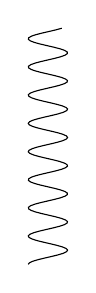
\begin{tikzpicture}
							\draw[domain=0:3,samples=150,variable=\y,black] plot ({cos(320*pi*\y+180)*0.25},{\y});
						\end{tikzpicture}
					\end{center}
			\end{columns}

			\begin{itemize}
				\item Acoustic energy is absorbed by tissue and causes deformation
			\end{itemize}
		\end{frame}

		\begin{frame}
			\frametitle{Sample ARFI Results}
			\begin{itemize}
				\item 4x4 of sample ARFI results
			\end{itemize}
		\end{frame}

		\begin{frame}
			\frametitle{ARFI Imaging Outcomes}
			\begin{itemize}
				\item ARFI more reliable than QS USE
			\end{itemize}
		\end{frame}

	\section[Shear]{Shear Wave Speed Quantification}
		\begin{frame}
			\frametitle{Introduction}
			\begin{itemize}
				\item QS USE and ARFI only provide \alert{qualitative} measures of stiffness
				\item Measuring shear wave speed allows quantifiable calculation of stiffness
				\begin{itemize}
					\item Can be used to accurately track over time and give absolute references
				\end{itemize}
				\item Uses ARFI pulses to generate shear waves in tissue
				\begin{itemize}
					\item Measure shear wave speed $\rightarrow$ calculate stiffness:

					\begin{equation*}
						c_T = \sqrt{\frac{\mu}{\rho}} \rightarrow \mu = c_T^2 \rho
					\end{equation*}
				\end{itemize}
			\end{itemize}
		\end{frame}

		\begin{frame}
			\frametitle{Measuring Shear Wave Speed}
			\vspace{1cm}
			\begin{enumerate}
				\item Induce ARFI at desired depth
				\begin{itemize}
					\item Shear waves radiate outward, like ``ripples in a pond''
				\end{itemize}
				\item Monitor deformation along a line extending from the focal point using B-mode
				\begin{itemize}
					\item Calculate speed of shear wave along this line
				\end{itemize}
			\end{enumerate}

			\begin{figure}
				\centering
				\begin{tikzpicture}
					\begin{axis}[
						scale only axis,
						enlargelimits=false,
						width=0.85\textwidth,
						height=3cm,
						xlabel={Time, $t$ (\si{\ms})},
						ylabel style={align=center},
						ylabel={Distance from \\ centerline, $x$ (\si{\cm})},
						axis on top]
							\addplot graphics[xmin=0,xmax=31.7,ymin=0,ymax=5]{../latex/assets/shear/data/lateralCut158.png};
							\addplot[draw=black, solid, ultra thick] table[x expr=\thisrow{t}*1000, y expr=\thisrow{x}*100] {../latex/assets/shear/data/shear_lateral_i158_isoline.dat};
							\draw[ultra thick, <->, draw=black] (axis cs:15,0.75) -- (axis cs:15,1.75);
							\draw[ultra thick, draw=black, dashed] (axis cs:0,0.75) -- (axis cs:17.5,0.75);
							\draw[ultra thick, draw=black, dashed] (axis cs:0,1.75) -- (axis cs:17.5,1.75);
							\node[right] at (axis cs:15,1.25) {Lesion};
							\draw[ultra thick, ->, draw=black] (axis cs:25.65,2.75) -- (axis cs:25.65,3.7755102040816);
							\node[below] at (axis cs:25.65,2.75) {Contour line};
					\end{axis}
				\end{tikzpicture}
			\end{figure}
		\end{frame}

		

	\section{Conclusions}
		\begin{frame}
			\frametitle{Experimental Validations}
			\begin{itemize}
				\item Experiments carried out using a \alert{Siemens ACUSON S2000\textsuperscript{\texttrademark}} ultrasound machine with a \alert{Siemens 9L4} transducer
				\item Used a \alert{CIRS QA Phantom 049} soft tissue model with stiffness-varying spherical lesions
				\item Compared parametrically-identical experimental results to simulation
				\item Got this ($\rightarrow$) characterization curve
				\item It works!
			\end{itemize}
		\end{frame}

		\begin{frame}
			\frametitle{Comparing Methods}
		\end{frame}

		\begin{frame}
			\frametitle{Recommendations}
		\end{frame}

	\appendix
	\section{Additional Slides}
	\setcounter{showProgressBar}{0}
	\setcounter{showSlideNumbers}{0}

		\begin{frame}
			\frametitle{Additional Slides}
			\begin{itemize}
				\item \hyperlink{backup1}{backup 1}
			\end{itemize}
		\end{frame}

		\begin{frame}[label=backup1]
			\frametitle{backup1}
			\begin{itemize}
				\item herp
			\end{itemize}
		\end{frame}

\end{document}